% !TeX root = ../main.tex

\chapter{个人贡献}

在此次大作业中,我负责研究可求解原问题 (\ref{problem}) 的算法、验证算法的可行性和使用 Python 语言实现算法 (\ref{Algorithm:RMFA}) 和算法 (\ref{Algorithm:DFAS}) 的原型并为组内其他成员提供基本的绘图框架。

\paragraph{算法研究}

通过观察如图 (\ref{Figure}) 的原问题 (\ref{problem}) 的函数和次梯度函数图像,不难发现,原问题 (\ref{problem}) 的解在它的次梯度函数图像上存在两种情况 \cite{10.1016/j.patcog.2017.02.006}:

\begin{enumerate}
    \item 解位于次梯度函数图像中一段函数与 $x$ 轴的交点;
    \item 解位于次梯度函数图像中的断点。
\end{enumerate}

\begin{figure}[htb]
    \centering
    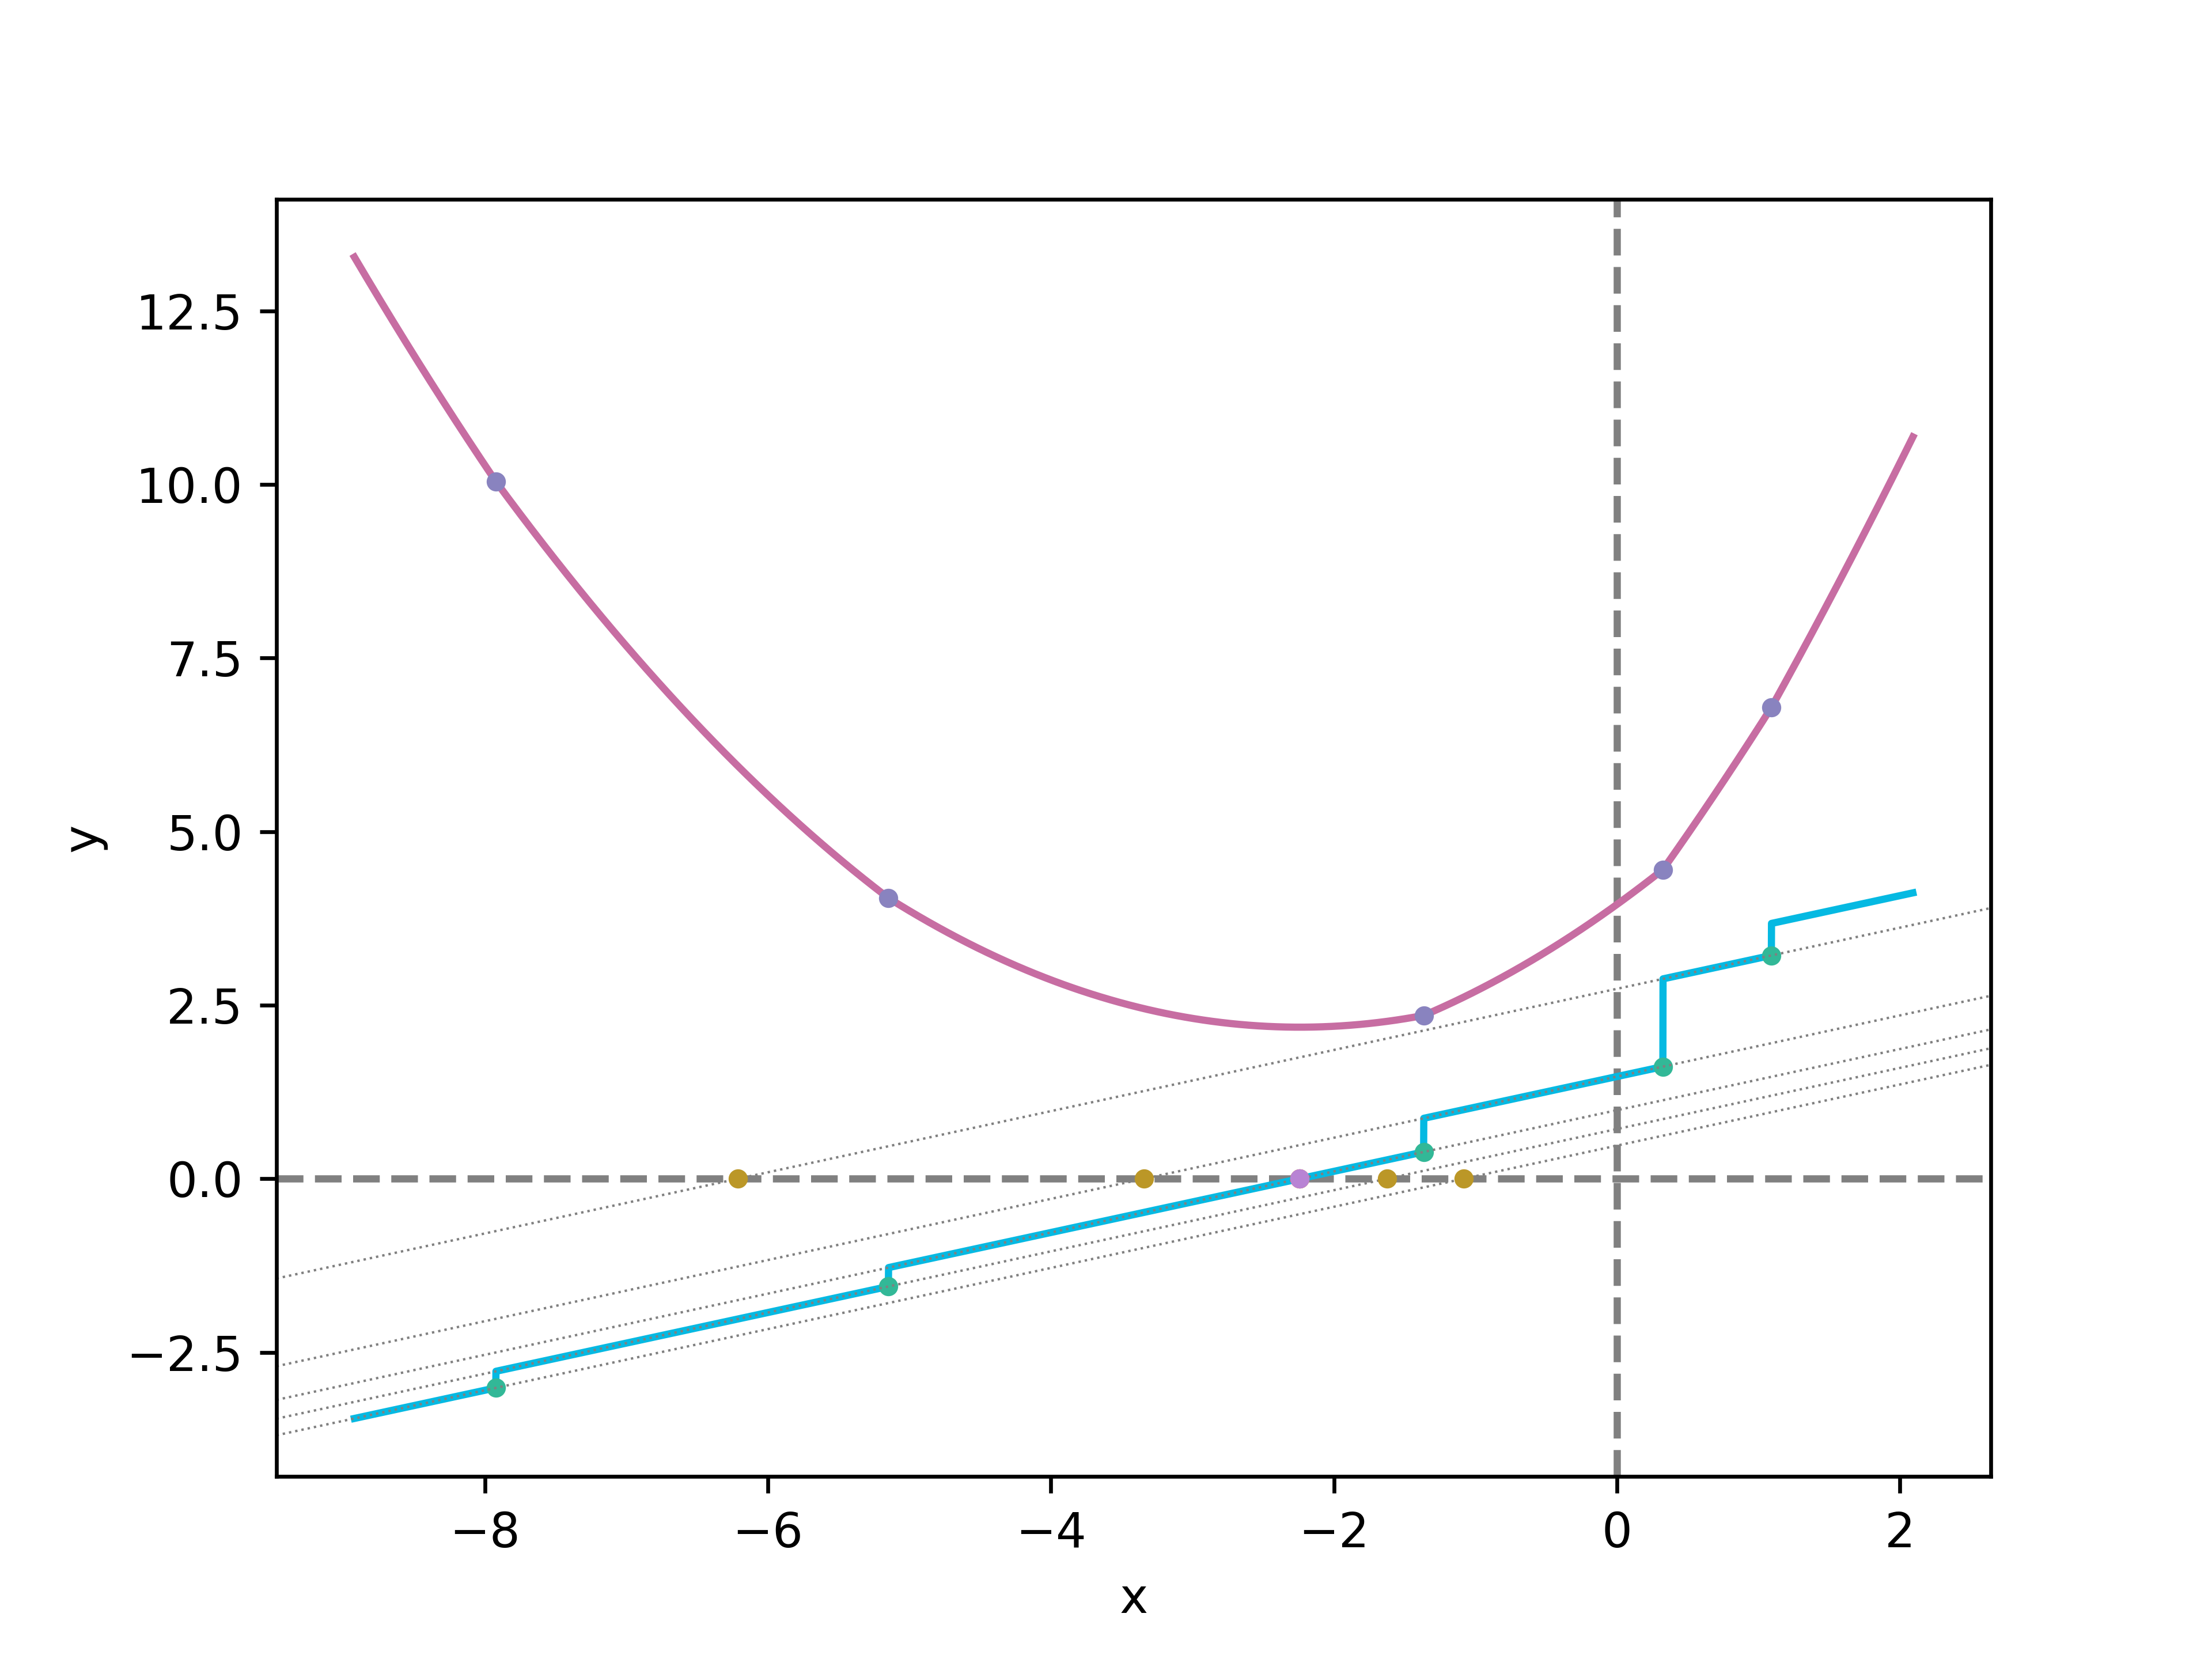
\includegraphics[width=0.45\textwidth]{figures/AxisX.png}
    \qquad
    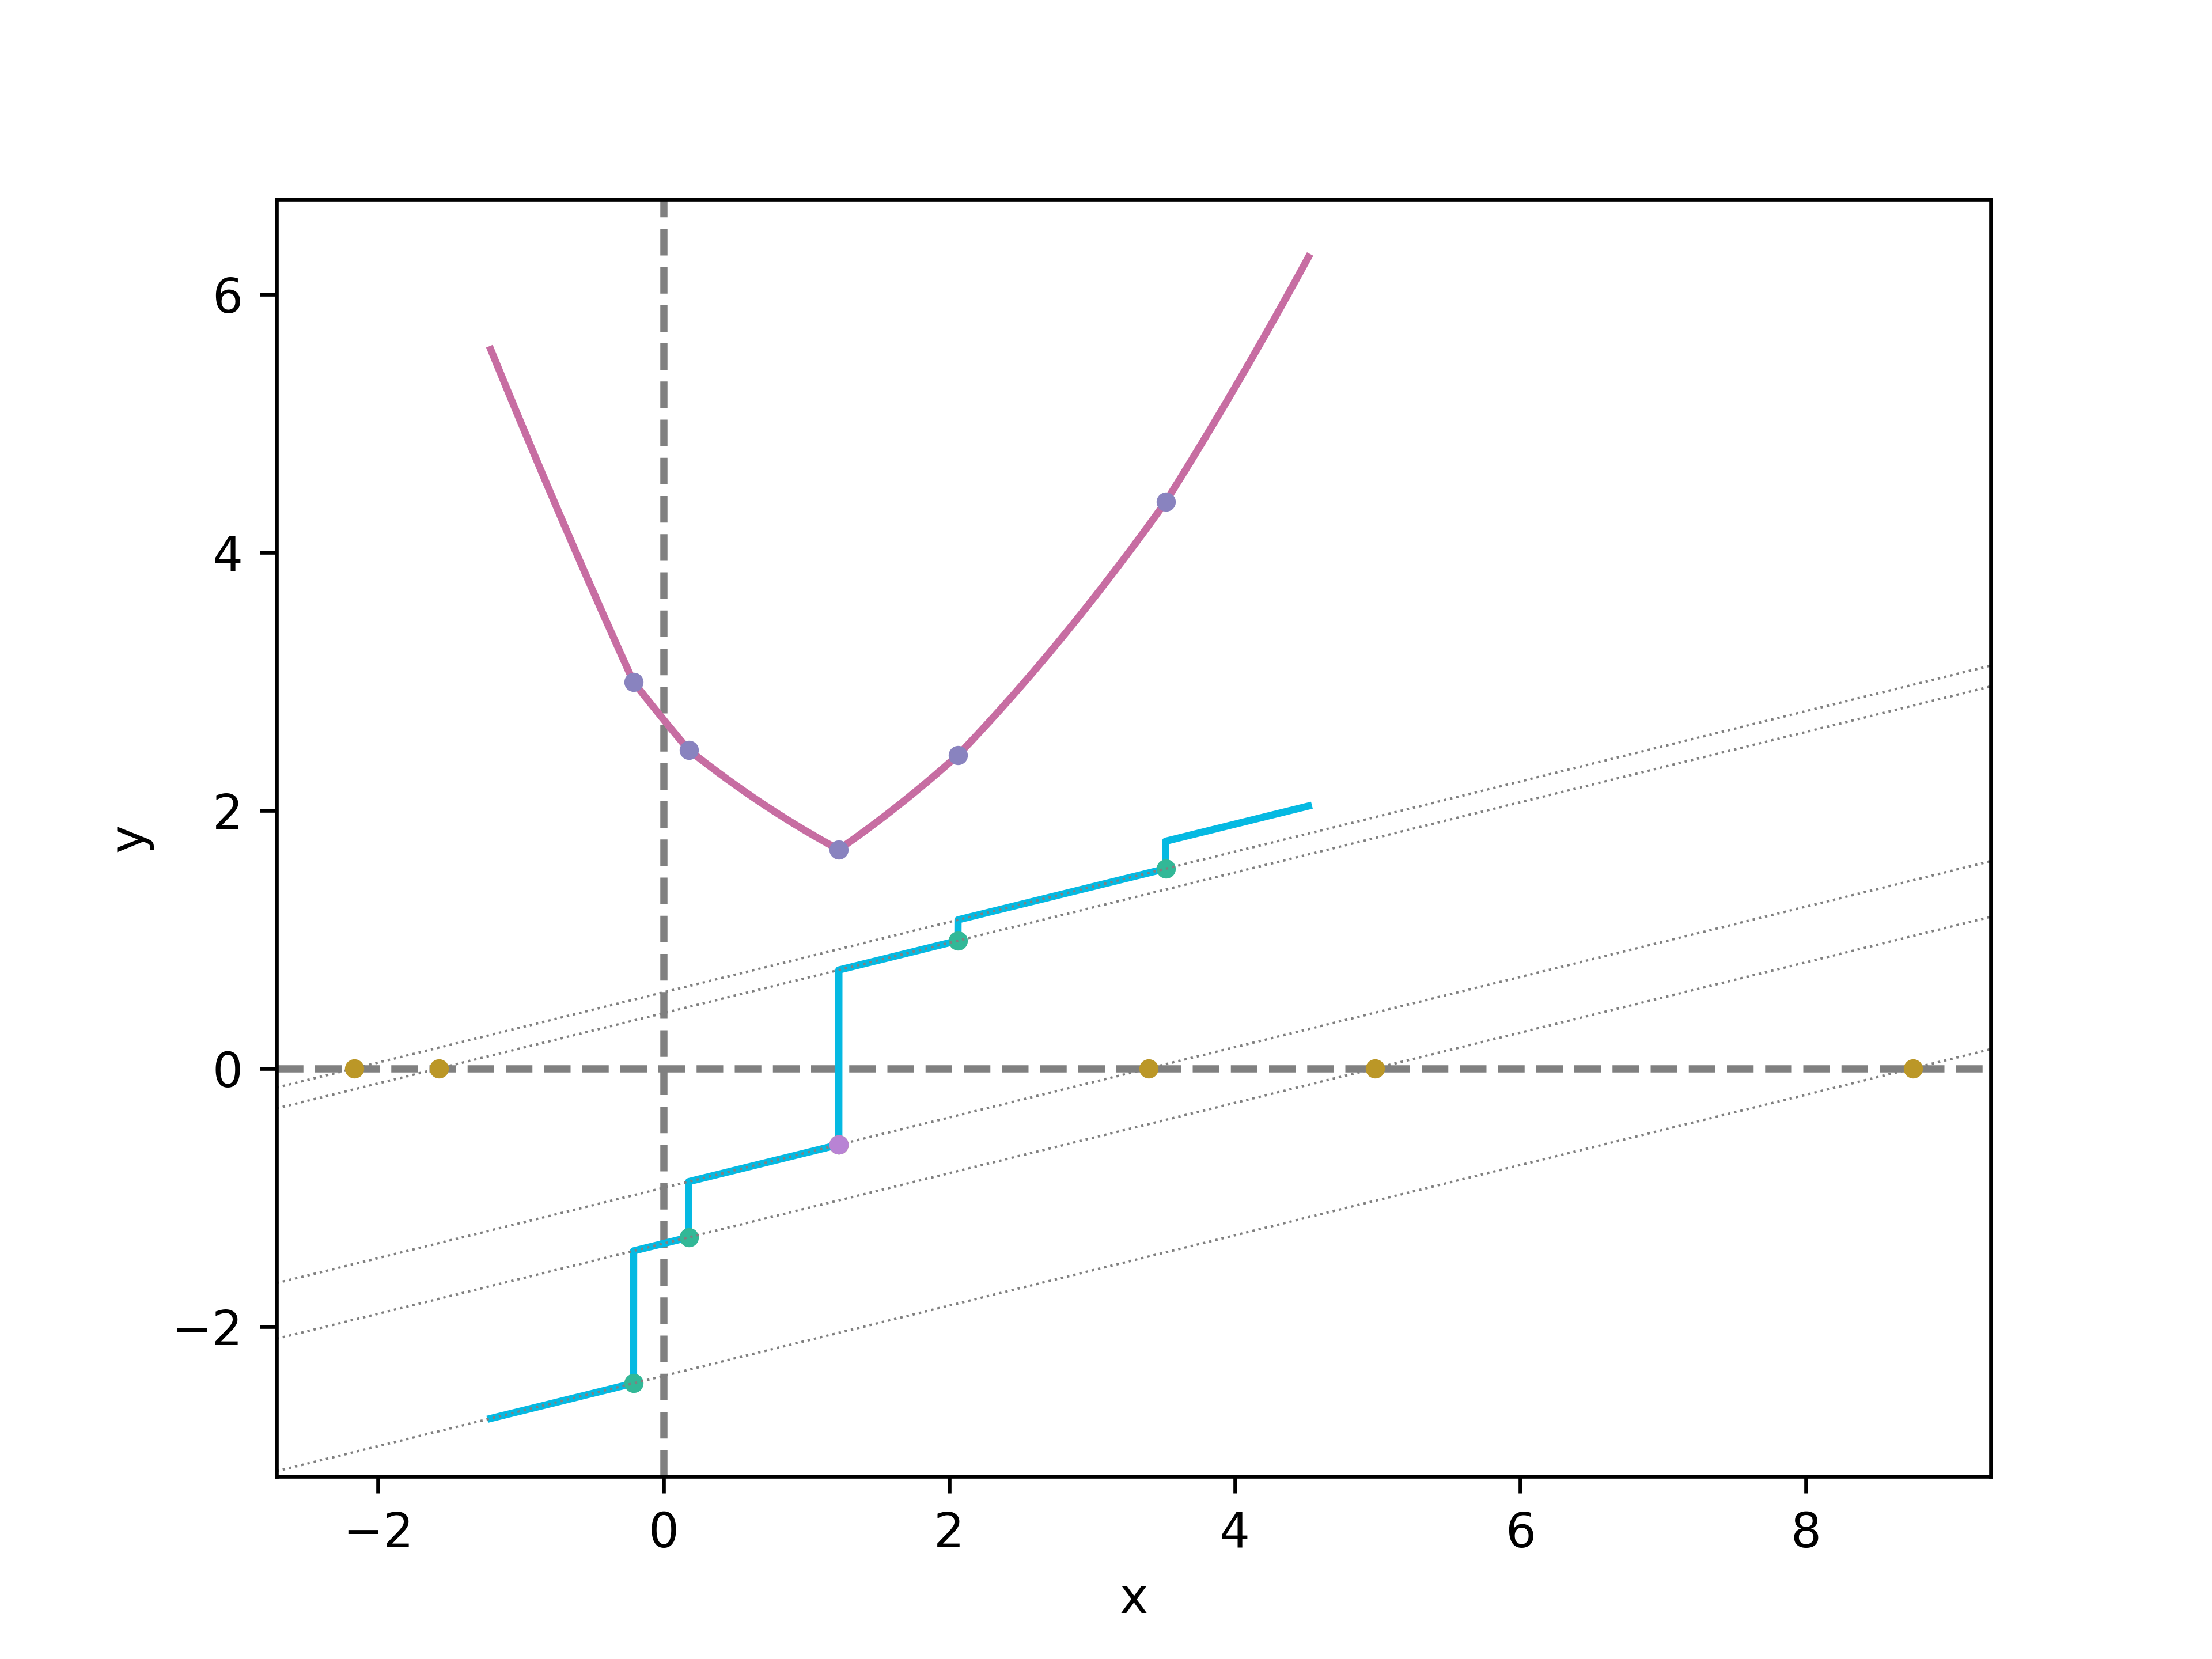
\includegraphics[width=0.45\textwidth]{figures/Breakpoint.png}
    \caption{位于 $x$ 轴上的解(左)和位于断点上的解(右)}
    \label{Figure}
\end{figure}

因此,在算法 (\ref{Algorithm:RMFA}) 和算法 (\ref{Algorithm:DFAS}) 中,也同样将问题分解为两种情况进行求解。譬如在算法 (\ref{Algorithm:RMFA}) 中,第 9 行便是针对解位于次梯度函数图像中的断点这一情况进行求解、第 16 行则是针对解位于次梯度函数图像中一段函数与 $x$ 轴的交点这一情况进行求解的。

\paragraph{算法实现}

在进行对上述两个算法的实现中,可以发现精度对算法正确性有着不小的影响,不确定的精度会影响断点的位置,使得断点或在上、或在下,如图 (\ref{Wrong}) 所示。
\begin{figure}[htb]
    \centering
    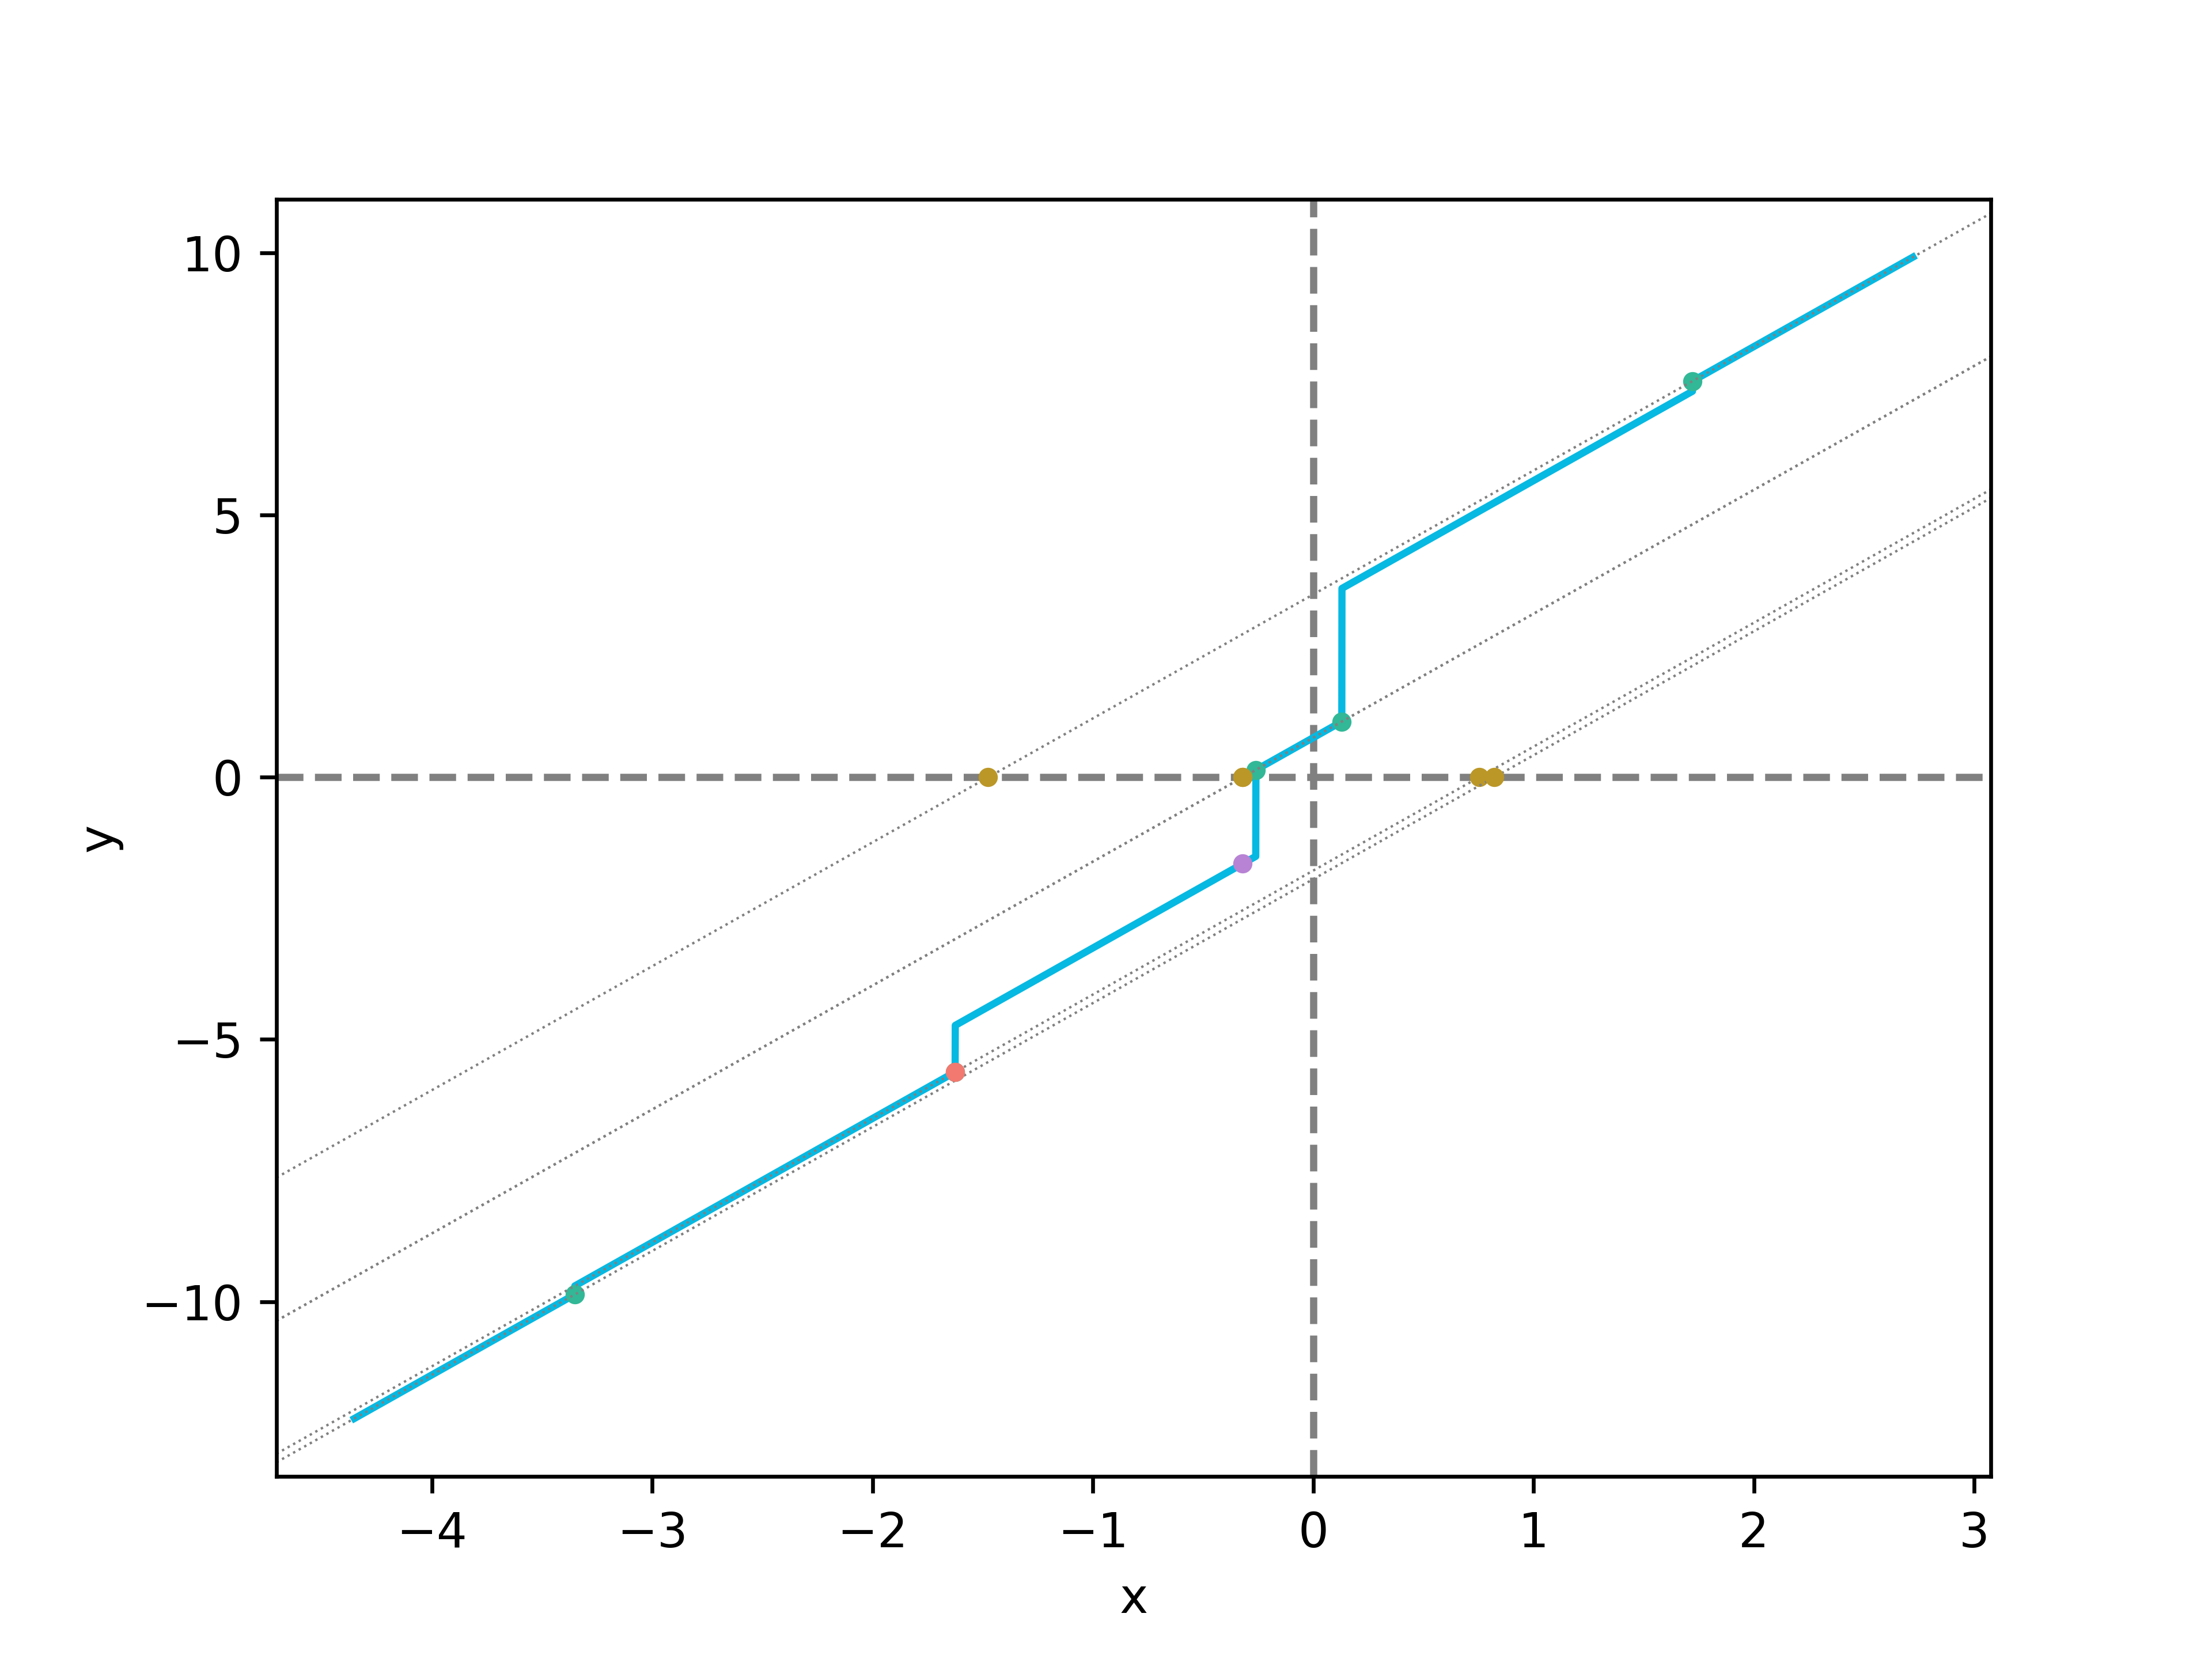
\includegraphics[width=0.5\textwidth]{figures/Wrong.png}
    \caption{错误的次梯度函数图像}
    \label{Wrong}
\end{figure}

可以看到,在图 (\ref{Wrong}) 中,断点(绿色点)的位置并非确定的在上方或下方,而是或上或下。两个算法所求的解也均不正确,算法 (\ref{Algorithm:RMFA}) 所求的解(紫色点)偏上,算法 (\ref{Algorithm:DFAS}) 所求的解(红色点)偏下。其对应的正确的次梯度函数图像如图 (\ref{Correct}) 所示,所有的断点应当统一在上方或下方,两个算法所求的解在图中也应当重合。

为了解决这个问题,首先要固定断点的位置。要固定断点的位置,一种简单的方法是:令精度为 $10^{-8}$,对每个断点向 $x$ 轴负半轴偏移 $10^{-8}$,即:
\begin{equation}
    x=\{x_i-10^{-8}|x_i=-\frac{c_i}{b_i},i=1\dots m\}\nonumber
\end{equation}

此时,所有的断点均被固定于下方,如图 (\ref{SubGradient}) 和图 (\ref{Answer}) 所示。在固定断点的位置后,再次使用算法 (\ref{Algorithm:RMFA}) 和算法 (\ref{Algorithm:DFAS}) 进行求解便可以得出正确的结果,如图 (\ref{Correct}) 所示。
\begin{figure}[htb]
    \centering
    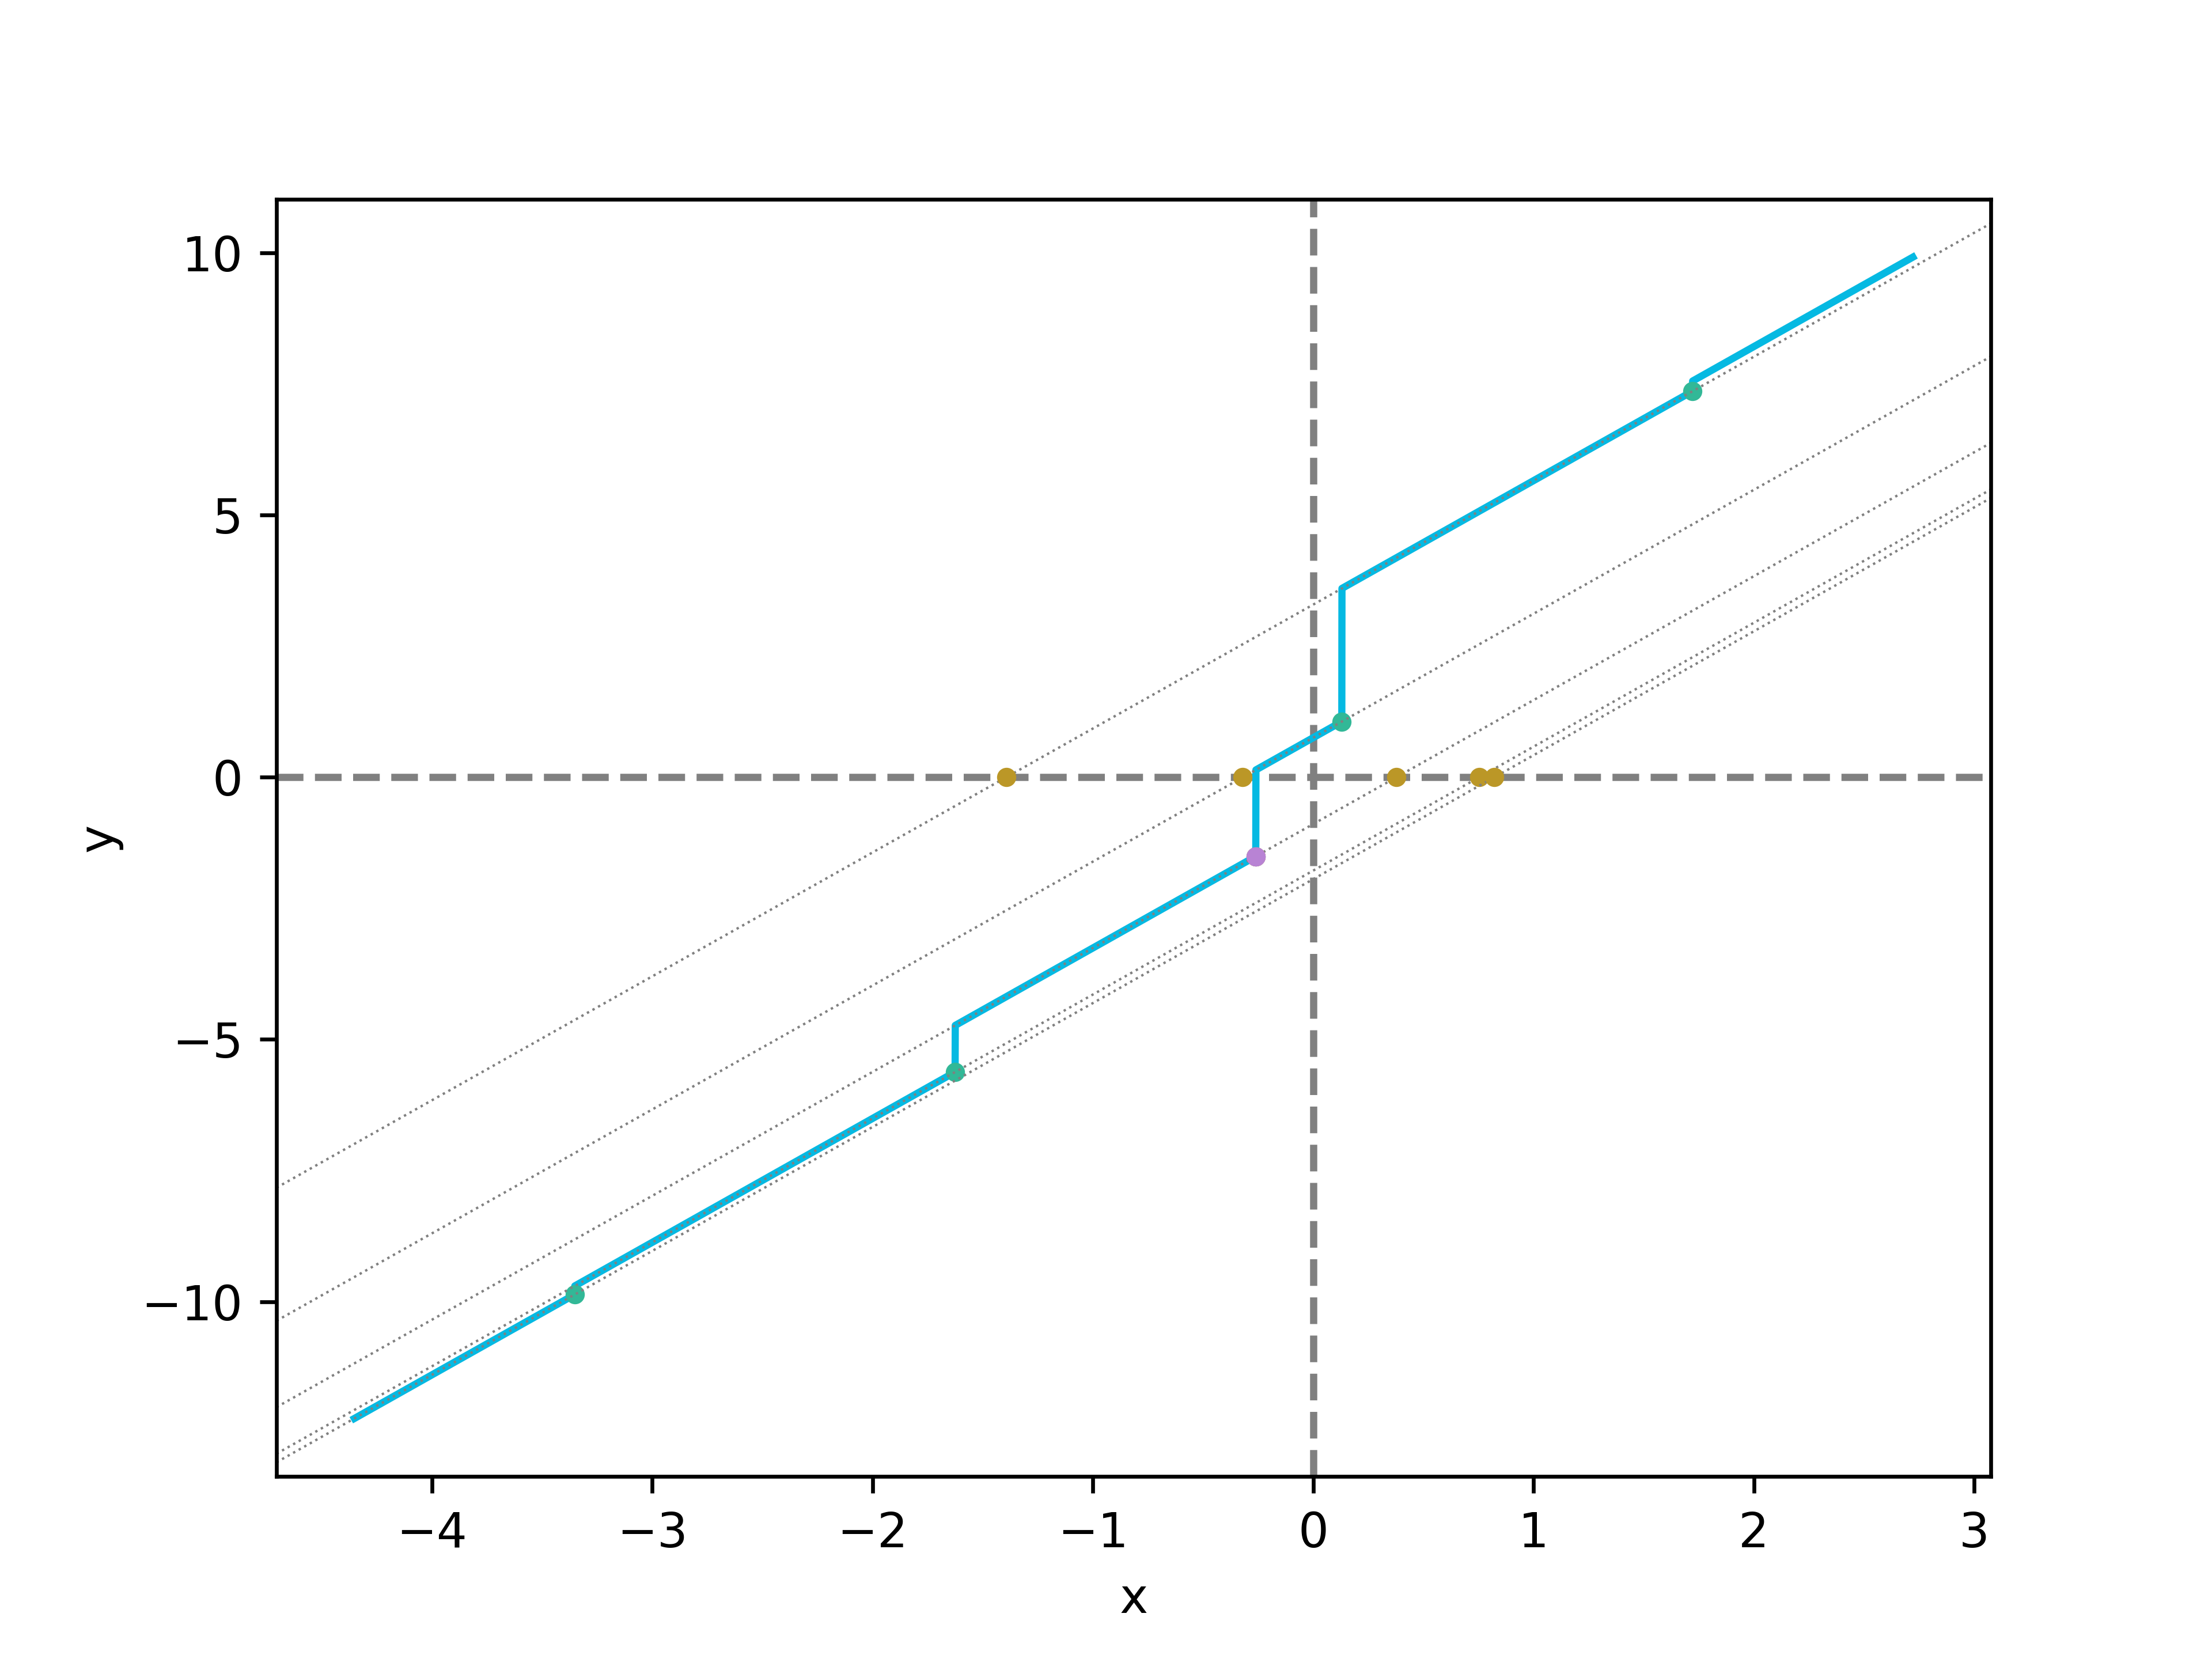
\includegraphics[width=0.5\textwidth]{figures/Correct.png}
    \caption{正确的次梯度函数图像}
    \label{Correct}
\end{figure}

Python 语言实现的算法原型代码已经上传至 \href{https://github.com/xqm32/unix-report-python}{https://github.com/xqm32/unix-report-python},仓库中还包含了组内其他成员编写的性能对比、图像绘制的代码。